\chapter{The Final Solution}
\label{chp:5:FinaSolu}
In this chapter, a final design of a mass communication system named Myriad will be introduced. To begin with, improvements on the requirements will be compared to those defined for the prototype from the previous chapter. Later on, the actual product features, its architecture, and the benefits of the final solution will be discussed in the conclusion.

\section{The Improved Requirements}
\label{sec:5.1:ImprRequ}

Seeing the prototype in action made us realize the need to revise the requirements and bring new ones. Some of those requirements are shaped according to the feedback we got during our research at the Stanford \ac{HCI} group, as well as from a Stanford organization who conduct mass email communication regularly in reaching their community. The following section will discuss those new features for the final product.

\subsection{Assistant Support}
\label{subsec:5.1.1:AssiSupp}
As described in section \ref{subsec:4.1.1:Cust}, the standard we want to achieve within a mass email communication is the most adequately personalized emails for every individual recipient, with a minimum effort on the researcher's side. The initial idea, as well as the prototype, included several features for this purpose, as discussed in chapter \ref{chp:4:InitIdeaProt}. However, considering the gold standard we would like to achieve as shown in figure \ref{fig:ChartEffortCustom}, the prototype manages to still leave an amount of effort on the researcher's side in accomplishing a successful mass email campaign.
\vspace{1cm}

In order to reduce the effort as much as possible during a mass email communication, the addition of an assistants' involvement was considered. Therefore, a primary researcher will be able to share tasks with permitted assistants. These might be tasks such as extracting information from the incoming answers, proofreading the primary researcher's replies before sending them, or even writing replies to those answers. Therefore, the primary researcher will only need to interact with the flow of a mass email campaign when the situation calls for it. However, the system would still need to provide necessary features that will be seen in the next sections in support for the workflow in a mass email campaign, hence, assistants will only need to interact with this workflow in letting the email campaign carry on by providing answers with using the provided email templates and extract information as \ac{KVP}s.

\subsection{Dynamic Variables and \ac{KVP}s}
\label{subsec:5.1.2:DynmVariKVPs}
We introduced the use of dynamic variables at the initial prototype; however, it was only limited to the salutation of the email. As described in section \ref{subsec:3.3.3:EmaiMarktAppl}, email marketing applications support this feature. And because it makes the personalization of emails easier, the final product will also include this feature. As a result, application users can create \ac{KVP}s and use the said keys in the content of an email message to be replaced dynamically by its value, according to the recipient. Therefore, the extracted information from emails will not just help us gather information in an organized way, but also in personalizing the emails.
\vspace{1cm}

As a result, instead of storing the \ac{KVP}s in the system according to their respective responses, the system should store them according to the recipients itself. This is where the \ac{KVP}-idea differs from the prototype. With this, we now have profiles of contacts for a campaign having all \ac{KVP}s of a recipient visible during the whole state of the conversation. However, the system should offer an option to hide individual \ac{KVP}s to avoid cluttering the view, and make the actively used \ac{KVP} list the default view.

\vspace{1cm}
Importing \ac{KVP}s can be done in several ways. One option is that the system should be able to synchronize with an online spreadsheet, e.g. Google Spreadsheet, in obtaining the \ac{KVP}s at the beginning of a campaign. This is a convenient way for researchers, since they are already familiar with spreadsheet environments. Other options should include a campaign-wide view and a contact specific view in the system. Also, it should have an editable keys and values in a campaign.

\subsection{Importing and Exporting Contacts and Their Information}
\label{subsec:5.1.3:ImpoExpoContInfo}
In the prototype, the application user has to enter all the basic information of the recipients such as first name, last name, and email address into the system manually. However, as they perform this, they use a spreadsheet and copy the contact information from there. This was also done for their regular email client used for email campaigns. The applications that were reviewed in section \ref{sec:3.3:Resul} all had an option to import data from spreadsheets to ease the process. Therefore, the system should also offer an option similar to this in importing contact information.
\vspace{1cm}

However, importing should not only be limited to the basic information of the recipients. Since we already mentioned about importing \ac{KVP}s from a spreadsheet in the previous section, the system should also be able to detect and import contact information and \ac{KVP}s related to a specific recipient, granting that they are available in the provided spreadsheet. 
\vspace{1cm}

The system should provide a bi-directional synchronization, and not just to import data from the spreadsheet. Therefore, the system should provide an option to export contact information and their created \ac{KVP}s from the system to the spreadsheet as well. This gives a reporting functionality to the application users, where they can see all of their recipients, and the extracted information from a specific campaign, all in one view.

\subsection{Interoperability with Other Email Clients}
\label{subsec:5.1.4:InteEmaiClie}
Even though we provided a new system for the users in initiating their mass email communication, there might be other cases wherein a mass email communication was initiated using a regular email client, therefore the system is not aware such campaign, since it was not created with it. The application should be able to provide an option in importing email messages created with a different email client into the system by recognizing specific messages, as annotated by the user.
\vspace{1cm}

Allowing the system to import email conversations from other email clients reduces the need for dependency on the application, and while researchers continue on using their own email clients, assigned assistants can take care of those emails, as imported by the researchers. We saw the same import feature in \ac{CRM} applications present in section \ref{subsec:3.3.1:CRMAppl} as well, where a user can easily forward an email to the \ac{CRM} application's provided unique email addresses, and the system then takes care of assigning the imported emails to the corresponding recipients in the system.

\subsection{Automated Decision-Making and Notifications}
\label{subsec:5.1.5:AutoDeciMakiNoti}
Even though the involvement of assistants helps make the primary researcher's life easier, the system still needs to provide an automated approach in answering emails whose statuses are clear in terms of its mass email communication flow. Therefore, a rule based decision-making mechanism should be used, at which a user sets the value of the keys from \ac{KVP}s, and it triggers the action of sending emails to qualified respondents whose \ac{KVP}s satisfies the provided condition.
\vspace{1cm}

Since the only purpose of the application is managing mass email communication and each campaign results to a great amount of messages in the inbox, the system should be able to provide notifications regarding what should be done next for each recipient. Labels should be added to email conversations to indicate whose turn is the next in the communication. For an instance, by proving a label saying "You need to reply" to the application user, the state of the communication awaits for an ample action from a researcher, or an assistant. In the same way, unread conversations and conversations waiting for an answer from the recipients should also be annotated in the appropriately. The system should also provide email notifications to the assistants' email addresses, to notify them whenever there is an action waiting to be taken care of.

\section{Final System}
\label{sec:5.2:FinaSyst}
In this section, we will see how the revised and improved requirements from the previous section reflected on the final product, named "Myriad".

\subsection{Log-In and Campaigns Overview}
\label{subsec:5.2.1:CampOver}

Similar to the prototype featured in section \ref{subsec:4.2.2:ProtSyst}, Myriad also requires a Gmail account to work with. The reason behind this is not just the popularity of Gmail, but also given the fact that Stanford University uses Google Apps by default, university wide. Therefore, each member of the university has a Google account ready to use with Myriad. This also provides flexibility, because Myriad does not have a registration form or a sign in screen. All the requested Google's permissions from a Myriad's user and their descriptions can be found in appendix \ref{app:GoogPerm}.
\vspace{1cm}

After users sign in to the system, the first screen they will see is the campaign overview screen. All created campaigns, including the ones assigned by other user's as an assistant are shown as in figure \ref{fig:CampaignsOverviewScreen}. It has a simple and clean \ac{UI}, compared to regular email clients, emphasizing its focus on mass email communication.

\begin{figure}[htbp]
	\centering
	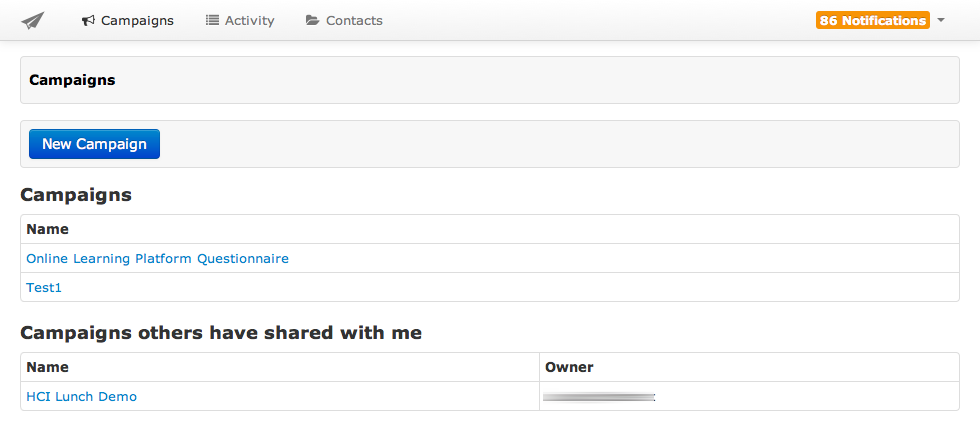
\includegraphics[width=1.00\textwidth]{imgs/CampaignsOverviewScreen.png}
	\caption[Myriad's Campaigns Overview Screen]{Myriad's Campaigns Overview Screen}
	\label{fig:CampaignsOverviewScreen}
\end{figure}

\subsection{Synchronization with Other Systems}
\label{subsec:5.2.2:SyncOtheSyst}

Myriad has the ability to get the recipients' information and their \ac{KVP}s from Google Spreadsheet\footnote{https://docs.google.com/spreadsheet/}. This is a convenient way in importing recipients' information into the system, since many people already keep their recipients' and related information in a spreadsheet environment as discussed in section \ref{subsec:5.1.3:ImpoExpoContInfo}. Therefore, Myriad offers a bi-directional syncing from and to a spreadsheet, as defined at beginning of the creation of a campaign. Besides this, Myriad also has an option to enter a recipient's first name, last name, and email address into the system directly.
\vspace{1cm}

The corresponding columns in a Google Spreadsheet start with "first name", "last name", and "email address" as shown in figure \ref{fig:GoogleSpreadsheet}. The rest of the columns will be filled out as a \ac{KVP}, and imported into the system as well.

\begin{figure}[htbp]
	\centering
	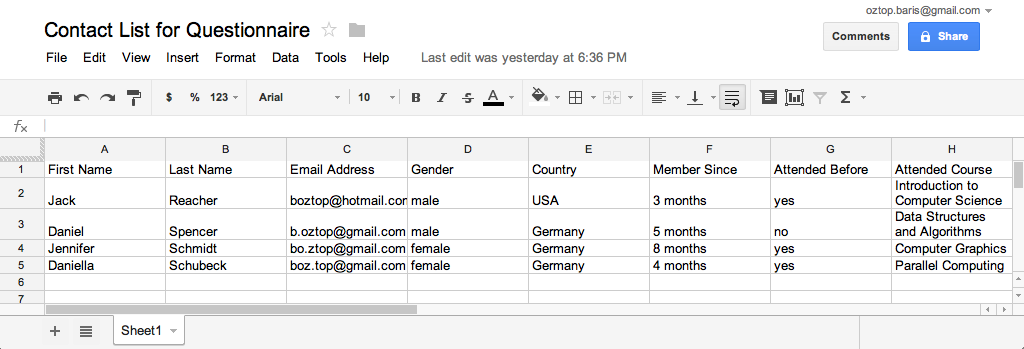
\includegraphics[width=1.00\textwidth]{imgs/GoogleSpreadsheet.png}
	\caption[A Google Spreadsheet to Import Recipients' Information into Myriad]{A Google Spreadsheet to Import Recipients' Information into Myriad}
	\label{fig:GoogleSpreadsheet}
\end{figure}

As mentioned in section \ref{subsec:5.1.4:InteEmaiClie}, importing existing email conversations as a campaign message into the system is an important feature. Researchers might have initiated conversations using their regular email client, and if later on they decide to make them more manageable, they can import them to Myriad. Myriad takes advantage of Gmail's labeling feature, which is equivalent to the \ac{IMAP} protocol's folders for the same purpose \citep{GoogleInc.2013}. Myriad creates a Gmail label in the user's account, and the only thing a user needs to do is the enable the label syncing feature at the campaign creation screen. Next, there will be a label similar to the campaign's name, and grouped under the root label, "myriad" in the Gmail's inbox (see figure \ref{fig:GmailLabels}). Hence, researchers will able to import email messages not considered a part of a campaign for some reason, into Myriad.

\clearpage

\begin{figure}[htbp]
	\centering
	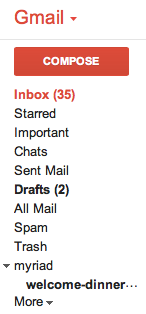
\includegraphics[scale=0.60]{imgs/GmailLabels.png}
	\caption[Gmail's Labels and Myriad's Campaigns Under the Myriad Label]{Gmail's Labels and Myriad's Campaigns Under the Myriad Label}
	\label{fig:GmailLabels}
\end{figure}

\subsection{Creating an Email Campaign}
\label{subsec:5.2.3:CreaEmaiCamp}

The campaign creation screen (see figure \ref{fig:CreateCampaign}) has input fields for a campaign name and Google Spreadsheet's \ac{URL} to synchronize with. Other two checkboxes for the spreadsheet are used to manage the frequency of synchronization and disabling the cascading warning messages in case of an erroneous data in the spreadsheet such as an empty email address field for a contact. The option for importing emails from Gmail's inbox is also in this screen, labeled as "synching section".

\begin{figure}[htbp]
	\centering
	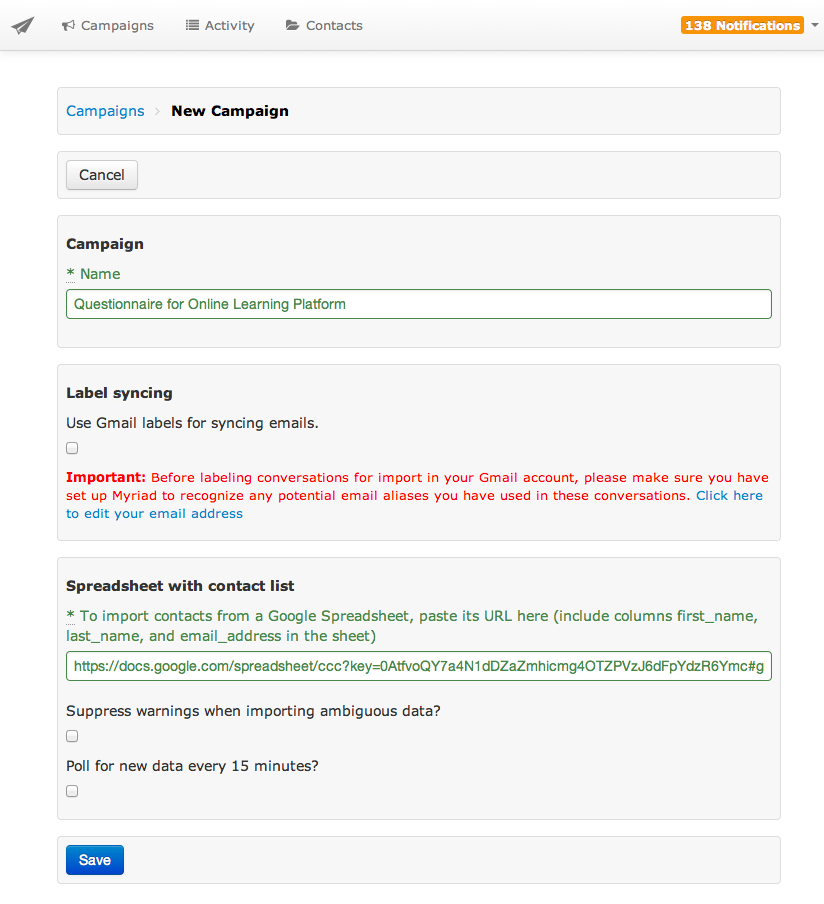
\includegraphics[width=1.00\textwidth]{imgs/CreateCampaign.png}
	\caption[Creating a Campaing in Myriad]{Creating a Campaing in Myriad}
	\label{fig:CreateCampaign}
\end{figure}

After the campaign is created, all the contacts and their \ac{KVP}s will be imported as long as the user provided a Google Spreadsheet \ac{URL} like in figure \ref{fig:ContactListInCampaign}.

\begin{figure}[htbp]
	\centering
	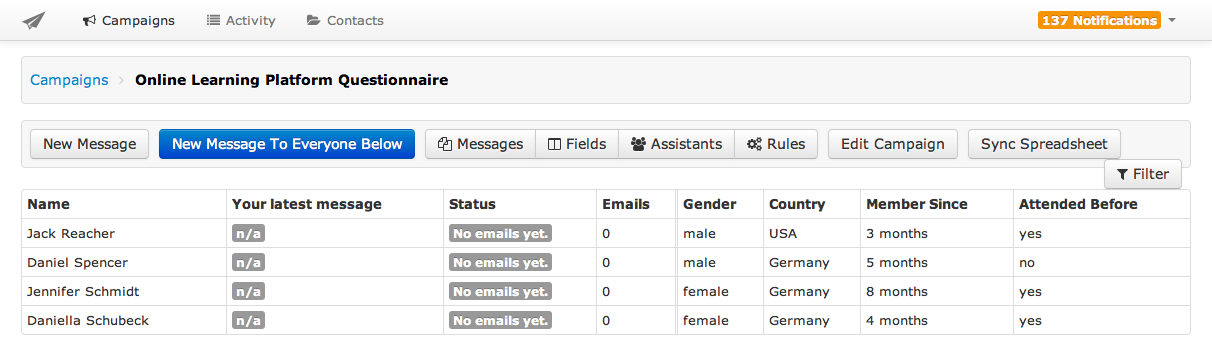
\includegraphics[width=1.00\textwidth]{imgs/ContactListInCampaign.png}
	\caption[Contacts and Their \ac{KVP}s After Synchronization in Myriad]{Contacts and Their \ac{KVP}s After Synchronization in Myriad}
	\label{fig:ContactListInCampaign}
\end{figure}

\clearpage

\subsection{Composing an Email Message}
\label{subsec:5.2.4:CompEmaiMess}

Users can send emails to all of the contacts they entered or imported into the system, or select a subset of them by using the filtering function as shown in figure \ref{fig:ContactFilters}. Provided filtering options are according to the values of \ac{KVP}s, the conversation statuses such as unread, replied, or unreplied, or the message's template names.

\begin{figure}[htbp]
	\centering
	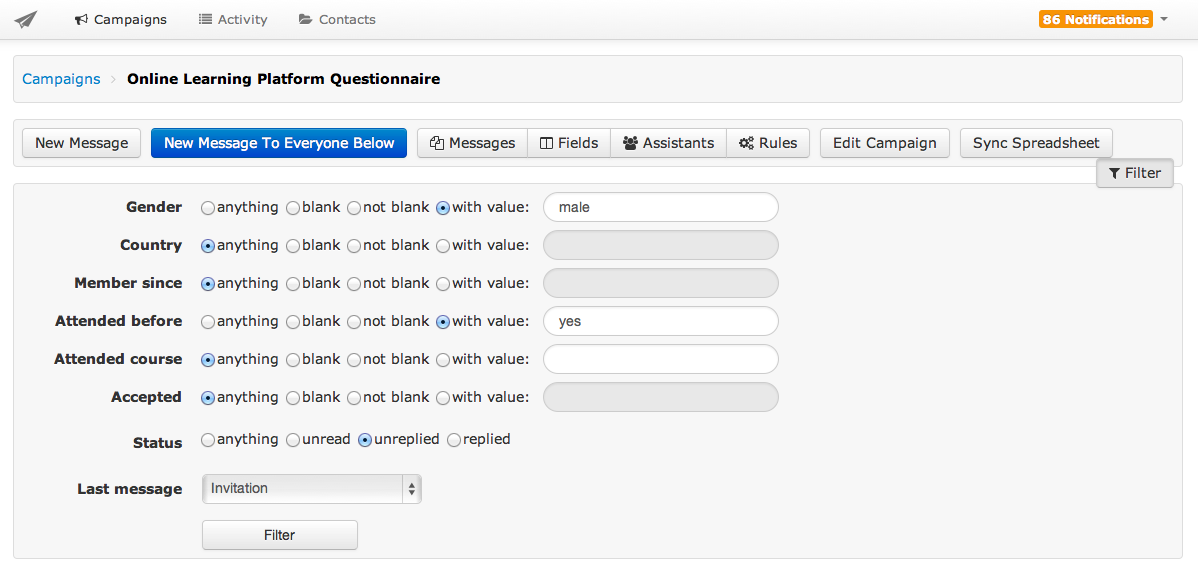
\includegraphics[width=1.00\textwidth]{imgs/ContactFilters.png}
	\caption[Filtering the Contact List in Myriad]{Filtering the Contact List in Myriad}
	\label{fig:ContactFilters}
\end{figure}

By pressing the corresponding button, users can now readily compose emails for their filtered recipients at the compose screen. The compose email pane (see figure \ref{fig:ComposeEmail}) contains a section that lists previously sent emails available for reuse. This is the same template concept that was introduced for the prototype in Chapter \ref{chp:4:InitIdeaProt}. Section \ref{subsec:4.2.2:ProtSyst}. It also shows the visualization of the flow of the communication by using a tree structure, as well as the number of messages sent by using the corresponding template. A more long term campaign's visualization tree can be found in appendix \ref{app:VisuCommStat}. The system also suggests an email template while composing a reply by considering the nodes at the same tree structure.

\begin{figure}[htbp]
	\centering
	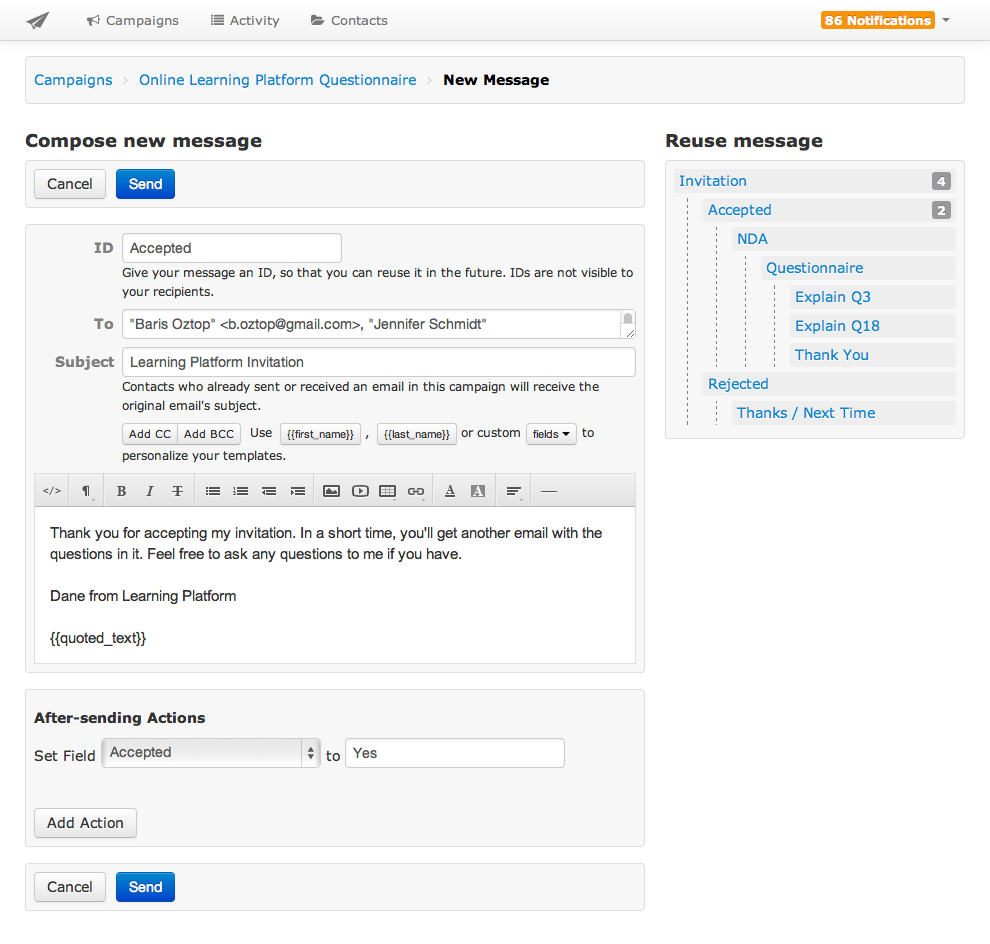
\includegraphics[width=1.00\textwidth]{imgs/ComposeEmail.png}
	\caption[Compose an Email in Myriad by Reusing Earlier Messages]{Compose an Email in Myriad by Reusing Earlier Messages}
	\label{fig:ComposeEmail}
\end{figure}

The compose pane allows users to add dynamic variables in the content of messages to personalize them according to the recipients. These variables are not just limited to the first name and last name, as they can also be of any keys from the assigned \ac{KVP}s in the campaign.
\vspace{1cm}

\clearpage

Each campaign has a link to the other campaigns, as ling as the recipient is involved in both campaigns, as featured in the next section. A researcher can access conversations and \ac{KVP}s from other campaigns by switching to the campaign via the provided link. Providing an option to see the earlier campaigns a recipient got involved in gives broader knowledge about a recipient that may help researchers in personalizing the content of the emails more easily and properly. For example, if we have extracted information regarding which sports did the recipients got involved with in an earlier campaign. We can use the same information in making a friendlier and to frankly start a new campaign by mentioning details about the latest events of those sports areas in the country. Such a technique also supports the social exchange theory and the diffusion of responsibility theory as discussed in section \ref{sec:2.3:PersEmai}. There is also an option to hide the \ac{KVP}s in a campaign if they are not related at all or have become obsolete during the flow of a campaign to avoid cluttering the application's view.
\vspace{1cm}

In figure \ref{fig:ComposeEmail}, at the pane of "after-sending actions", users are able to set the values of the keys right after an email is sent. Therefore, a user does not need to browse to another screen in order to change or set \ac{KVP}s whose values depends on the email that was recently sent.
\vspace{1cm}

At the beginning of this section it was mentioned that a user can filter the recipients list, and then send an email to a subset, according to the filter's criteria. Myriad saves those filtered criteria under the "Rules" menu as shown in figure \ref{fig:AutomatedRules} after the user sent the email. Therefore, the next time the system receives new emails with the same conditions as before, user will see them under the rules menu, and the earlier sent email messages can be sent to those new matching recipients automatically, if user opt to enable the automated response feature or a user can simply press the send button manually in the same screen. For example, in figure \ref{fig:AutomatedRules}, there are three recipients whose "attending" key were set to "yes", and since the system already recognized that we have already sent an email to those attending, new matches for the same condition applies. In this case, the user can simply press the send button, or automate the process by enabling the provided option.

\clearpage

\begin{figure}[htbp]
	\centering
	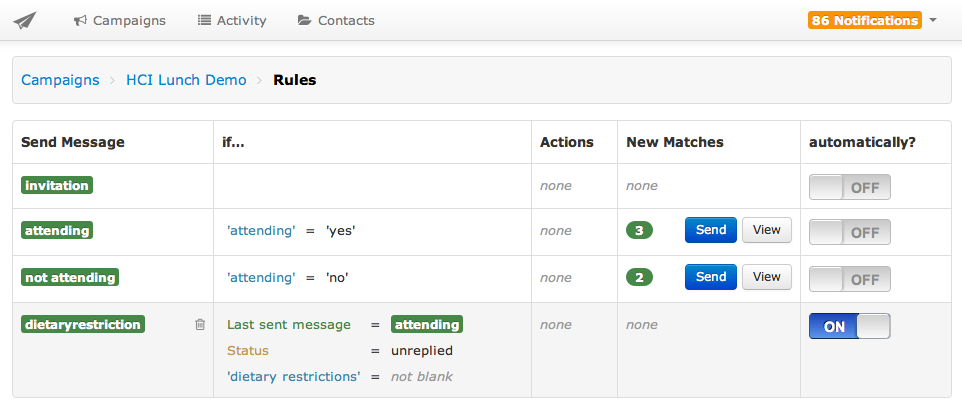
\includegraphics[width=1.00\textwidth]{imgs/AutomatedRules.png}
	\caption[Rules to Automate the Sending Process of the Emails in Myriad]{Rules to Automate the Sending Process of the Emails in Myriad}
	\label{fig:AutomatedRules}
\end{figure}

\subsection{Extracting Information from Email Messages}
\label{subsec:5.2.5:ExtrInfoEmaiMess}

Myriad's reading pane (see figure \ref{fig:MyriadReadingPane}) offers a threaded view wherein all of the messages between a specific recipient and a researcher are visually grouped together. The advantage of a threaded view is that it allows a researcher to get a quick overview of the whole state of a conversation, therefore a researcher can write a customized message more easily by focusing on the specific personality of the individual being responded to, considering earlier conversations with him or her at a single glance.
\vspace{1cm}

Each of the researcher's message is annotated with the name of the message template that was used with, making the latest state of the communication easily recognizable without having to look for its content. In figure \ref{fig:MyriadReadingPane}, emails sent by the user have green labels with indicators of the name of the template used, such as "Accepted" and "Invitation".
\vspace{1cm}

While reading a recipient's answer, the extracted information can be recorded as \ac{KVP}s at the right-hand side of the reading pane (see figure \ref{fig:MyriadReadingPane}). Earlier recorded keys' values can also be updated at the same pane. Having \ac{KVP}s along with the conversation thread gives the researcher necessary information about the person being replied to. Under the \ac{KVP}s pane, the researcher can also see if the recipient is involved with another campaign, and a link to the involved campaigns are provided with the number of emails exchanged, next to it. This is a helpful feature in reminding researchers about the existence of previous interactions with the recipient, and if necessary, the researcher can switch to other campaigns to get an overview of extracted information as \ac{KVP}s.

\begin{figure}[htbp]
	\centering
	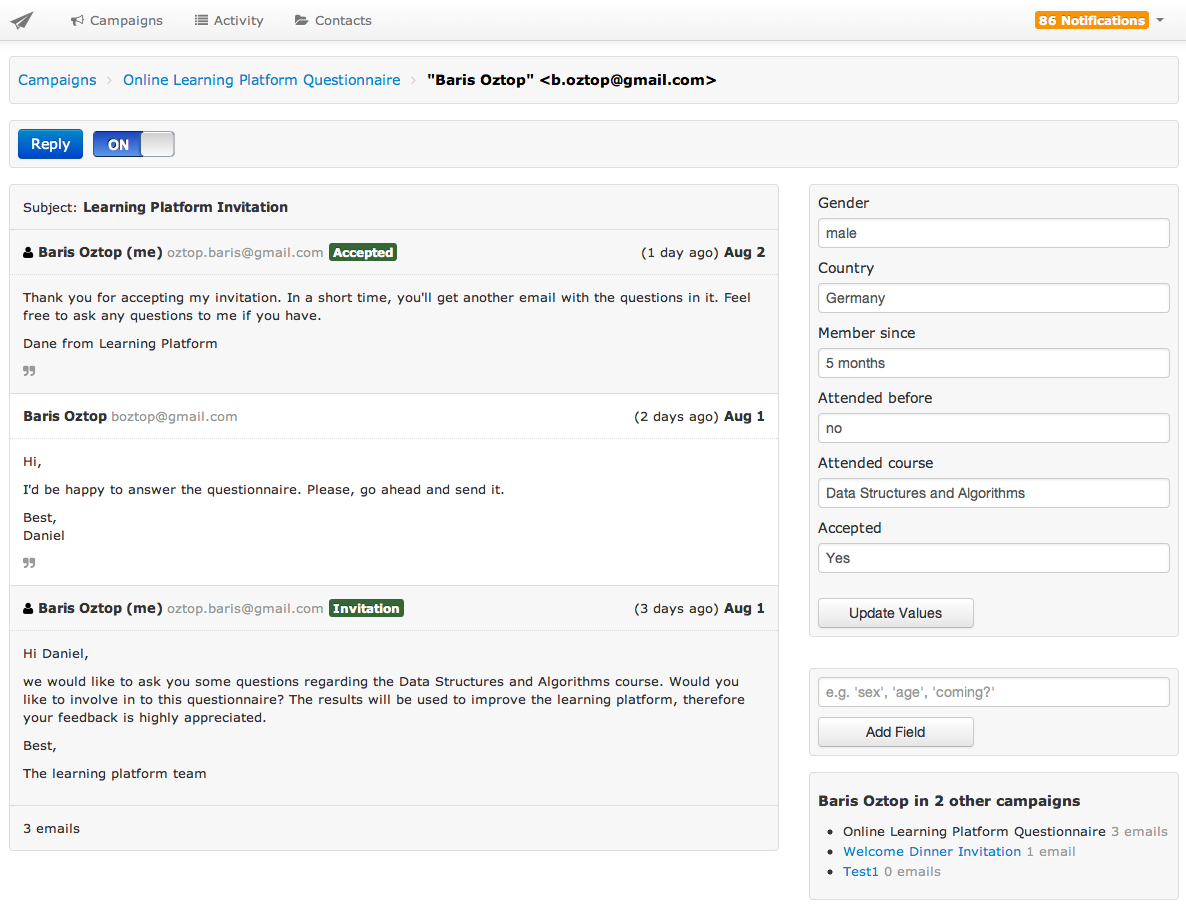
\includegraphics[width=1.00\textwidth]{imgs/MyriadReadingPane.png}
	\caption[The Reading Pane and the Extracted \ac{KVP}s in Myriad]{The Reading Pane and the Extracted \ac{KVP}s in Myriad}
	\label{fig:MyriadReadingPane}
\end{figure}

\subsection{Enabling Assistants}
\label{subsec:5.2.6:EnabAssi}

A researcher can add other researchers as assistants into a campaign by adding their Google account associated email addresses into Myriad, as shown in figure \ref{fig:AddAssistants}. The task of the assistant can range from extracting information from emails, writing answers to the recipients, to proofreading a researcher's emails before sending them, and many other tasks that can be generated according to the type of help a researcher needs.

\clearpage

\begin{figure}[htbp]
	\centering
	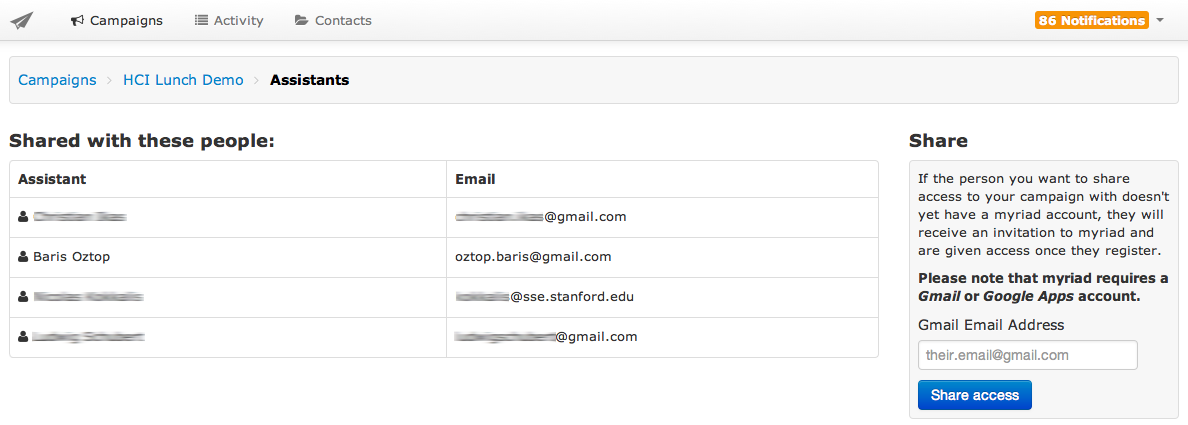
\includegraphics[width=1.00\textwidth]{imgs/AddAssistants.png}
	\caption[Rules to Automate the Sending Process of the Emails in Myriad]{Rules to Automate the Sending Process of the Emails in Myriad}
	\label{fig:AddAssistants}
\end{figure}

After an assistant is assigned to a campaign, he or she will get a notification email including the link to the campaign. Again, there will be a notification email for each email sent by a respondent to the assistants' email address to let them know that they need to act on the situation.
\vspace{1cm}

Myriad provides status labels for each received or sent email, giving a hint on the next awaiting action similar to what is shown in figure \ref{fig:EmailStatuses}. These status labels give hints about the next action to be taken according to the state of the conversation, such as if the user needs to read or to send a reply to a message, or the conversation awaits for an answer from the recipient's side to continue to the communication. There are also status labels related with Myriad's internal state regarding to an email message, such as if Myriad was able to send the messages successfully, or if there was a failure encountered while sending them. The same view also provides a column showing last message sent by the user. With this, the researchers and the assistants will easily realize what should be done next, and see the status of the communication for each recipient. 

\clearpage

\begin{figure}[htbp]
	\centering
	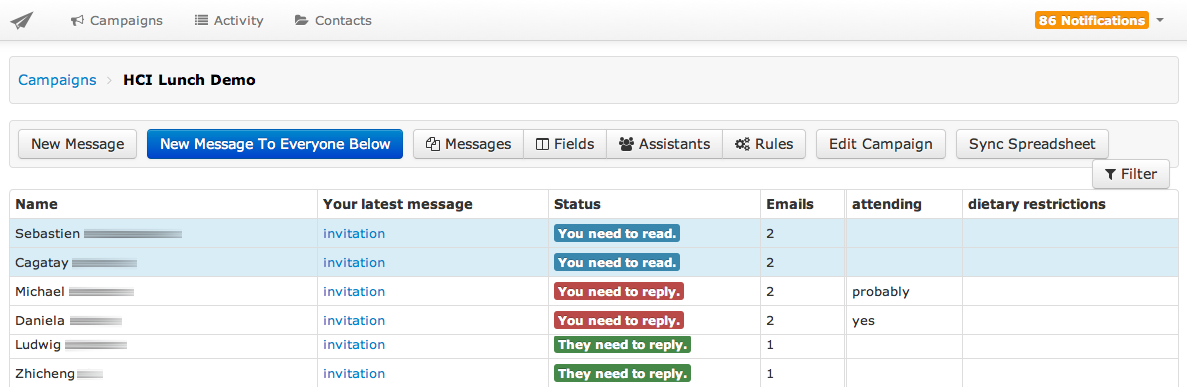
\includegraphics[width=1.00\textwidth]{imgs/EmailStatuses.png}
	\caption[Status Labels for Each Email in Myriad]{Status Labels for Each Email in Myriad}
	\label{fig:EmailStatuses}
\end{figure}

\section{Architecture}
\label{sec:5.3:FinaArch}

Similar to the prototype, Myriad was also developed using a framework stack of \ac{RoR}, jQuery, Bootstrap, and OAuth\footnote{OAuth is leveraged by using OmniAuth library (https://github.com/intridea/omniauth), and its Google authentication strategy is implementation by OmniAuth Google OAuth2. Details can be found at https://github.com/zquestz/omniauth-google-oauth2} protocol was used for the authentication with Gmail. The initial project structure was generated by a gem named Rails Apps Composer\footnote{https://github.com/RailsApps/rails\_apps\_composer}, consisting a collection of Rails application templates to start a project. Thanks to the other gems utilized for the project development and completing it on time in a robust way. The following section will discuss the implementation details of Myriad, how it makes mass email communication easier.

\subsection{Keeping Track of Recipients}
\label{subsec:5.3.1:ReciCont}

As mentioned in section \ref{sec:4.2:Prot}, the prototype was not able to keep the basic contact information of the recipients, only the messages of them. Therefore, extracted information such as \ac{KVP}s are only limited to email messages related to the recipients. The downside of this approach is its inability in obtaining all the \ac{KVP}s of the recipients all at one glance. Instead, we need to go through earlier emails of the recipients each time we need to create the same key, since the system was not aware of an existing \ac{KVP} created for a different email in the same campaign.
\vspace{1cm}

In Myriad's case, this issue was solved by keeping all the recipients' information in a separate data model named "contact" as shown in figure \ref{fig:UML_Draw_Final}. With this, we were able to keep track of the recipients among different campaigns through different conversations involving them, which is another set of a data model in the Myriad system, as each campaign involves many conversations with the recipient involved with them.
\vspace{1cm}

Myriad keeps all of the basic profile information of the recipients, including their first names, last names, and email addresses. These information can be imported into Myriad either by spreadsheet synchronization, by adding them into "To" filed when a user composes an email, or by importing from Gmail's inbox via the label synchronization. The recipients' email addresses are unique identifiers for Myriad in order to compare already existing recipient information with the synchronized ones. 

\begin{figure}[htbp]
	\centering
	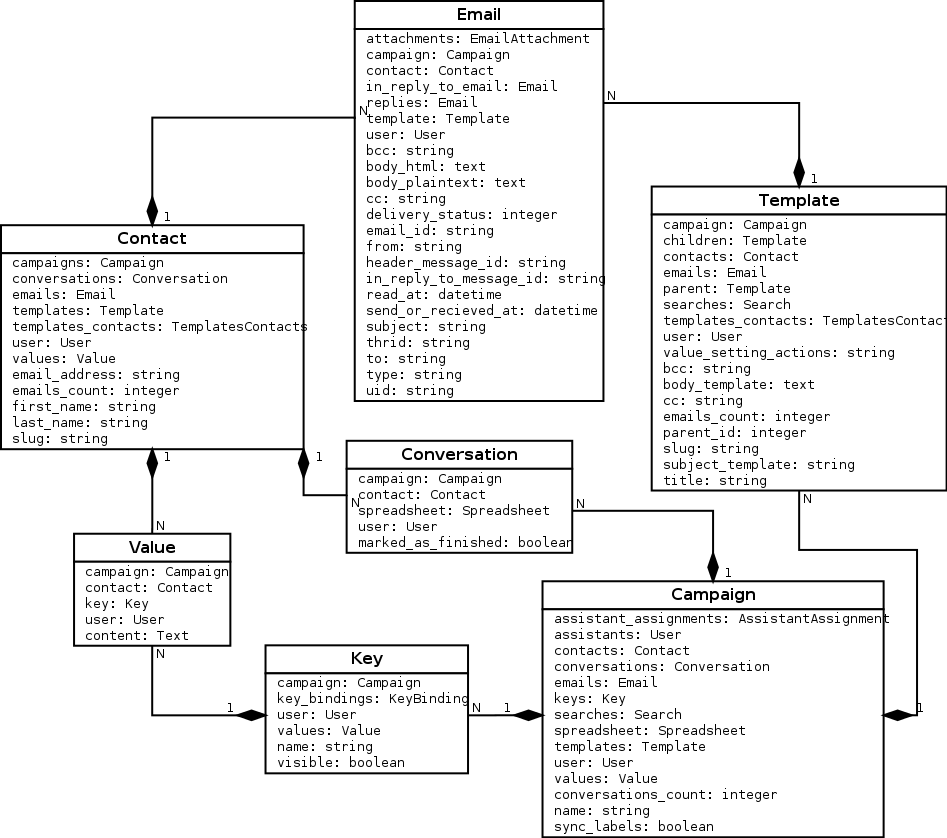
\includegraphics[width=1.00\textwidth]{imgs/UML_Draw_Final.png}
	\caption[Model Dependency of the Myriad Compared with the Prototype]{Model Dependency of the Myriad Compared with the Prototype}
	\label{fig:UML_Draw_Final}
\end{figure}

\subsection{The \ac{KVP}s and the Templates}
\label{subsec:5.3.2:KVPsTemp}

Having a separate contact data model in keeping track of the recipients also helped us relate extracted information, specifically \ac{KVP}s of the recipients, instead of their message in a campaign as shown in figure \ref{fig:UML_Draw_Final}. Each campaign has many keys, and as well as their corresponding values, according to the recipients. One advantage of this is that as we browse a specific conversation with a recipient, we will be able to see all \ac{KVP}s of the specific recipient under one view, which is the \ac{KVP} pane next to the email threads, as shown in figure \ref{fig:ComposeEmail}. The other benefit is its ability to synchronize with spreadsheets. When a new key is added to a recipient or a value of a key is updated via Myriad, it will be reflected on the spreadsheet as well. Therefore, the spreadsheet will always contain the latest changes done by the user in Myriad. 
\vspace{1cm}

Similar to the prototype, templates contain emails messages with dynamic variables in it, and the actual emails whose dynamic variables are filled with values are kept in the Email data model as shown in figure \ref{fig:UML_Draw_Final}, after they are fetched from Gmail.
\vspace{1cm}

To get an overview of the conversation and let the users select templates, Myriad offers a tree structure similar to the prototype. However, the execution of the tree structure is different from the prototype. In section \ref{subsec:4.2.3:ProtArch}, it was mentioned that the hierarchy between the nodes of the tree was a nested set model. We decided to use an adjacency list model instead of a nested set model to increase the readability of the templates' relationship with the data model level from the developers' perspective. Since the relation of the templates is not as complicated compared to hierarchical relations, the performance drawbacks on this decision was negligible.

\subsection{A Campaign Message Identification}
\label{subsec:5.3.3:MessIden}

Due to the prototype's dependency on the existing EmailValet's email fetching process, we identify emails if they belong to a specific campaign or are user's regular emails, and then inserting them into the same inbox in EmailValet. With Myriad, we removed this dependency, and considered showing emails belonging to a campaign.
\vspace{1cm}

The identification of the emails depends on the three different conditions:

\begin{compactenum}
	\item The emails fetched from Gmail and responses to one of to the campaign message.
	\item The emails composed in Myriad as a part of the campaign, whether they are the emails to initiate a campaign or replies to recipients' emails.
	\item The emails imported into Myriad from Gmail's inbox via label synchronization (as shown in section \ref{subsec:5.2.2:SyncOtheSyst} for label synchronization)
\end{compactenum}

Myriad initially retrieves all the email's \ac{UID}s\footnote{UID (Unique Identifier) is 32-bit integer value to uniquely identify emails in a mailbox in \ac{IMAP}. Each email added into mailbox will have a higher value than the ones added before, however they are not necessarily contiguous \citep{rfc3501}. \ac{UID} is used as it was in the prototype by the implementation of the EmailValet's part. It is used to identify if a message is already fetched from Gmail, if it is not, it is fetched since it is a new message.} from Gmail's inbox for the last 14 days, instead of all the emails in the inbox to reduce the time needed for the fetching process. For those \ac{UID}s not stored in the Email data model of Myriad, Myriad retrieves the actual email along with the metadata, such as Gmail thread ID\footnote{Gmail thread ID is a 64-bit integer that is part of the provided Gmail's IMAP extension. It helps to associate groups of messages in the same manner as in the Gmail web interface \citep{GoogleInc.2013a}.} and Gmail labels.
\vspace{1cm}

For the prototype, we have set a specific message-ID to the emails composed in Myriad. With this, we are able to identify whether an email from Gmail was composed to initiate a campaign or is a reply to one of the recipients of a campaign by a Myriad user during the aforementioned fetching process. Message-ID field is again leveraged for identifying a recipients' message belonging to a campaign. Myriad retrieves the Message-ID written in the In-Reply-To, and checks if it matches one of the campaign messages in Myriad. Another field that Myriad checks is the "References" field\footnote{Reference field in another identification field along with Message-ID defined by RFC 5322. It contains one or more Message-IDs used when creating a reply to a message to identify the original message or the other messages when a reply to a message that was itself a reply \citep{rfc5322}.} to identify messages as a part of a campaign, but was forwarded to another person by a recipient in order to reply the message. Since the forwarded endpoint's email client sets the Message-ID of the forwarded message into the In-Reply-To header field and sets a new Message-ID, Myriad is not familiar with neither of the Message-IDs at all after it got the forwarded or replied message. Myriad checks the "References" field to identify a Message-ID belonging to a campaign in this case. This scenario is illustrated in figure \ref{fig:drawingMessageReferences}.

\begin{figure}[htbp]
	\centering
	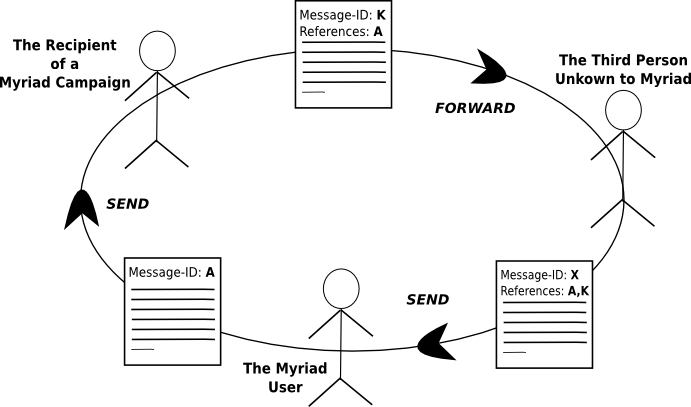
\includegraphics[width=1.00\textwidth]{imgs/drawingMessageReferences.png}
	\caption[A Scenario Using References Field in an Email]{A Scenario Using References Field in an Email}
	\label{fig:drawingMessageReferences}
\end{figure}

If an email is not identified as a part of a campaign message by comparing the Message-IDs with the ones in Myriad's Email data model, the next step is to evaluate those emails in case they are labeled as part of a Myriad campaign in Gmail's inbox. In this case, if an email has a label in the pattern of "myriad/campaign-name", and there is already a created campaign in Myriad with the name "Campaign Name", that email will be stored in the data model. Finally, an identified email will be assigned to a contact by looking at its parent email's Message-ID if it was a reply or if it fails, the contact information will be recorded from the email's "From" header field. The rest of the emails will be ignored if no matches were found in the mentioned email header fields, specifically Message-ID, In-Reply-To, and References, or Gmail's Label.

\section{Experiences}
\label{sec:5.4:Expr}

To date, Myriad has 67 users since its beta launch\footnote{Beta version of Myriad was launched at http://gv.stanford.edu/ and still accessible from this address.} last January 30, 2013. Among those 67 users, 30 of them are actively using it, since last month. In this section, statistics will be given about the created campaigns, and continued with some user's testimonials.

\subsection{Statistics}
\label{subsec:5.4.1:Stat}

The beta launch of Myriad has been advertised at the Stanford \ac{HCI} group and to some of Stanford's organizations who performs mass email communication regularly with their communities. Some of those campaigns opted to use the following features of Myriad, such as:

\begin{compactitem}
	\item \textbf{Invitation to an Event:} User created an initial invitation template and another template for those who rejected the invitation to motivate them for other upcoming events. Recipient list is imported via spreadsheet. User also created \ac{KVP}s to easily identify recipients needing an individual follow up. Salutations of the emails are personalized by their first name through \ac{KVP}s.
	\item \textbf{Survey via an External Link:} Users send an initial template including a link to an external survey. A detailed list of contact information was imported from a Google spreadsheet. Later on, users continued with a reminder email in a separate campaign.
	\item \textbf{Importing via Gmail Labels} One of the user imported campaign emails from his Gmail account to Myriad via a label synchronization, and continued the campaign in Myriad.
	\item \textbf{Interview Results} One user reached nearly 500 recipients through Myriad in releasing the result of an interview process. User created a rejection template for those who were rejected, and for the ones who were accepted, he created several templates depending on the invitation date, including the specific schedule related to that date. The user also automated the email sending process by the created rules on the filtered search results.
	\item \textbf{Getting User Details via Form} During one of the live demonstrations of Myriad at the Stanford \ac{HCI} group, we asked to the attendees to browse to a link and fill up a Google Form\footnote{https://docs.google.com/forms} to obtain their contact information in a Google Spreadsheet, where the gathered data is recorded in Google Form by default. Therefore, we were able to easily import contact information into Myriad, and initiate a campaign. There were also four assistants extracting information during the live demonstration while the recipients were sending answers.
\end{compactitem}
\vspace{1cm}

After reviewing some cases using Myriad in real time, the following paragraphs will provide usage statistics regarding Myriad, starting from its beta launch date, January 30, 2013 until August 7, 2013.

\paragraph{Campaigns and Their Number of Recipients} Figure \ref{fig:ChartCampaignsRecipients} shows campaigns\footnote{Campaigns' names are removed due to privacy reasons.} created by Myriad, and their respective number of recipients. The average number of recipients was 105.32, and the total number of recipients was 9585. While the maximum number of recipients for one campaign was 752, the minimum amount was only one recipient.

\begin{figure}[htbp]
	\centering
	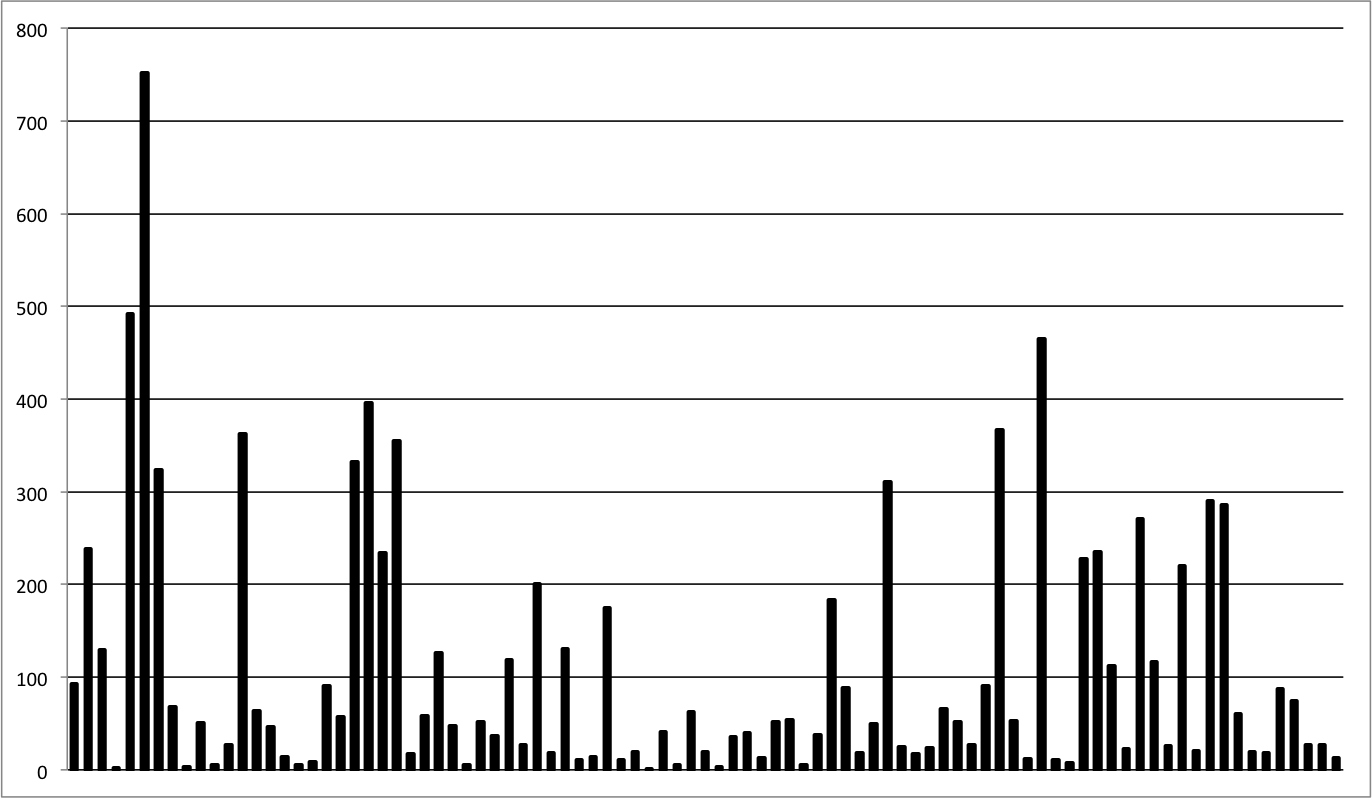
\includegraphics[width=1.00\textwidth]{imgs/ChartCampaignsRecipients.png}
	\caption[Campaigns and Their Number of Recipients in Myriad]{Campaigns and Their Number of Recipients in Myriad}
	\label{fig:ChartCampaignsRecipients}
\end{figure}

\paragraph{Myriad Users and Their Number of Campaigns} Figure \ref{fig:ChartUsersCampaigns} shows Myriad's total number of users\footnote{Users' names are removed due to privacy reasons.}, and the number of campaigns that they created with Myriad. There are a total 96 campaigns, after the ones created for test purposes were ignored. The average was 3.92 campaigns per user. While the maximum amount of campaigns created by one user was 13, the minimum amount was one campaign.

\begin{figure}[htbp]
	\centering
	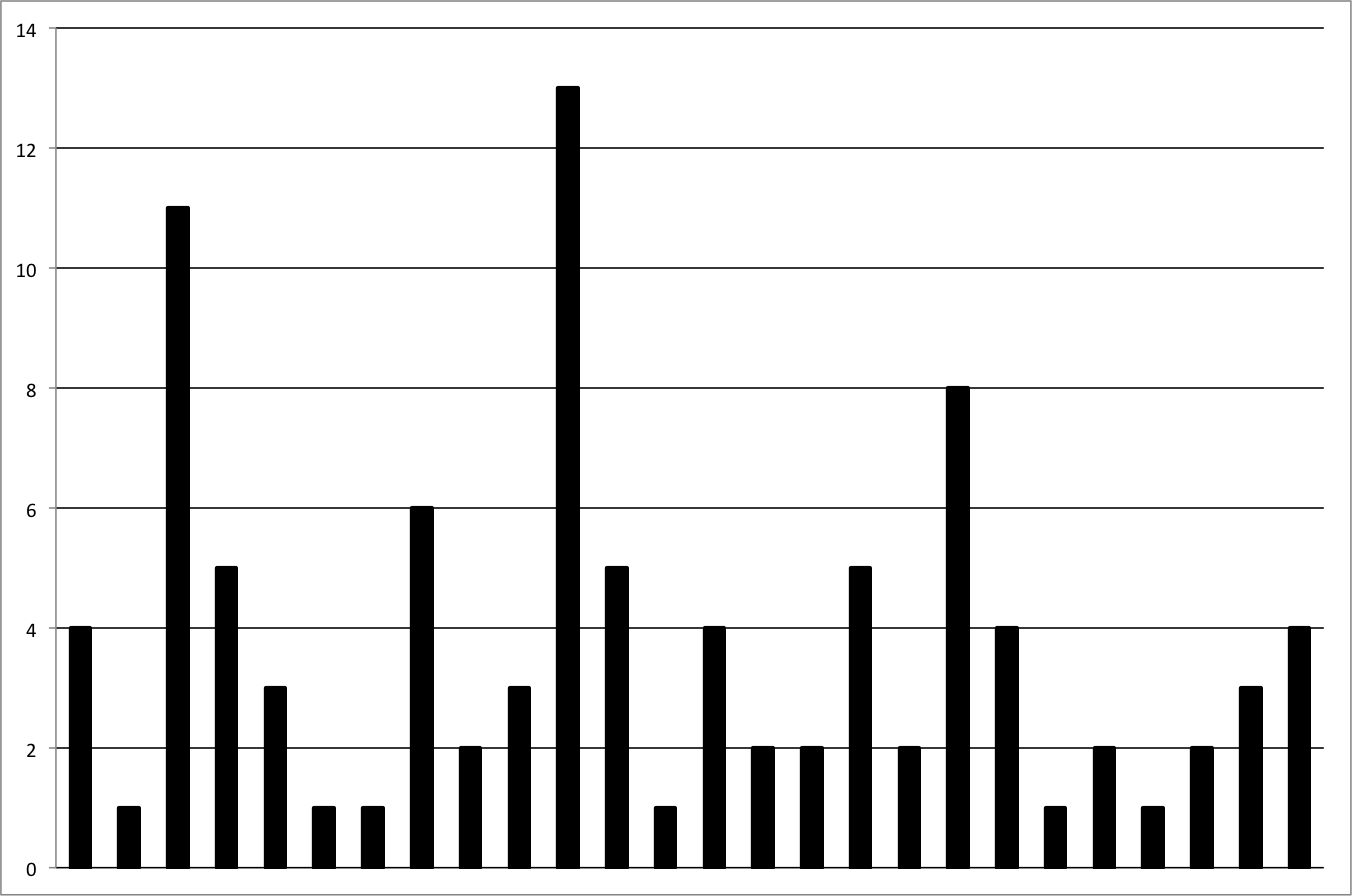
\includegraphics[width=0.85\textwidth]{imgs/ChartUsersCampaigns.png}
	\caption[Myriad Users and Their Number of Campaigns]{Myriad Users and Their Number of Campaigns}
	\label{fig:ChartUsersCampaigns}
\end{figure}

\clearpage

\paragraph{The Number of Campaigns per Month} Figure \ref{fig:ChartCampaignsMonths} shows the ratio of created campaigns per month. 35 campaigns out of 96 were created in April 2013, as the highest amount compared to other months. It might be because it is the middle of spring quarter at Stanford University, where lecturers and organizations need to reach their recipients more often. There were an average of 15.5 campaigns create per month if the launch month January is ignored.

\begin{figure}[htbp]
	\centering
	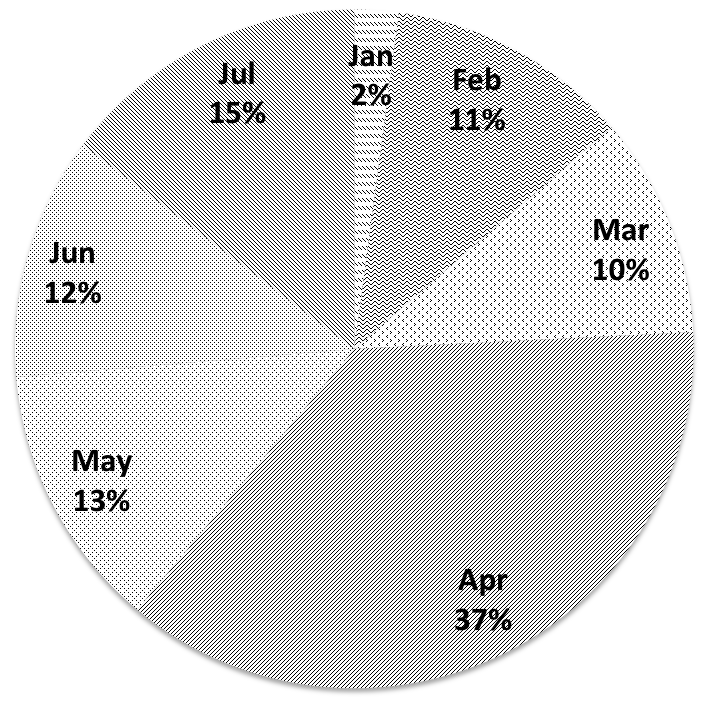
\includegraphics[width=0.50\textwidth]{imgs/ChartCampaignsMonths.png}
	\caption[The Number of Campaigns per Month]{The Number of Campaigns per Month}
	\label{fig:ChartCampaignsMonths}
\end{figure}

\subsection{User Testimonials}
\label{subsec:5.4.2:UserTest}

In this section, testimonials from the very active users of Myriad will be evaluated. Users were asked to evaluate Myriad, keeping the following four questions in mind:

\begin{compactenum}
	\item What are the scenarios you use Myriad for?
	\item What were you using before Myriad?
	\item How satisfied are you with Myriad?
	\item How regularly do you use Myriad?
\end{compactenum}

Testimonials written in listing \ref{lst:Testimonial1} and \ref{lst:Testimonial2} belongs to lecturers from the Stanford \ac{HCI} group. The last testimonial belongs to a Stanford organization who performs mass email communication very often to reach their community.

\vspace{1cm}

\clearpage

\lstset {
 basicstyle=,
 frame=shadowbox,
 rulesepcolor=\color{black},
 showspaces=false,showtabs=false,tabsize=4,
 numberstyle=\tiny,
 captionpos=b,
 xleftmargin=0.7cm, xrightmargin=0.5cm,
 lineskip=-0.1em,
 abovecaptionskip=1\baselineskip
}

\begin{lstlisting}[language=, caption={[User Testimonial \#1 about Myriad]User Testimonial \#1 about Myriad}, label={lst:Testimonial1}]

My main use: handling a special issue. Several hundred emails (literally) meant that an email view was impossible. Myriad's structured view makes everything a whole lot easier. It still needs some polishing to be ready for prime time (like it's workflow emphasis is a little constrained, and it needs better handing of formatting and attachments), but as a first draft, it's amazing. I hope it continues so I can use it more!

- Scott R. Klemmer, Stanford HCI Group
\end{lstlisting}

\vspace{1cm}

\begin{lstlisting}[language=, caption={[User Testimonial \#2 about Myriad]User Testimonial \#2 about Myriad}, label={lst:Testimonial2}]

I use Myriad to manage a large volume of emails about the courses that I'm teaching. I tag the email with the campaign, and the system+assistant help me respond with one of a number of common responses.

- Michael S. Bernstein, Stanford HCI Group
\end{lstlisting}

\vspace{1cm}

\begin{lstlisting}[language=, caption={[User Testimonial \#3 about Myriad]User Testimonial \#3 about Myriad}, label={lst:Testimonial3}]

I use Myriad when I'm mass-mailing a group of people and want to personalize the email. Before, I was using Mailchimp or BCC everyone. It's a great tool to send personalized emails to the network! I use Myriad whenever I need to email more than 10 people and want to personalize the emails. For less than 10, the set up for Myriad may take longer than sending out the emails individually (this was discovered through trial and error).
\end{lstlisting}

\section{Conclusion}
\label{sec:5.5:Conc}

In this section, the final solution, Myriad, for mass email communication was investigated. We first investigated the improved requirements, comparing them with the initial requirements, and the ones already applied to the initial prototype. Enabling assistant support, using \ac{KVP}s as dynamic variables in the email, importing recipients list from a Google Spreadsheet, the ability to import email from Gmail's inbox by annotating emails using Myriad's campaign labels, and automated decision-making through previously applied search filters were some of the main improvements done in Myriad.
\vspace{1cm}

Previous sections continued showing how those features were applied for Myriad's \ac{UI}, followed by introducing its architecture on how it was possible to enable the said features in support for mass email communication.
\vspace{1cm}

Finally, user and campaign statistics were given to show how actively Myriad was used during its beta stage, and the section was followed by testimonials from the active users of Myriad.
\vspace{1cm}

After discussing what Myriad is, its features, and users' testimonials, let us see how these features fit into a personalized mass email communication. A personalized mass email communication can be illustrated as shown in figure \ref{fig:drawingStatesOfEmailCommunication}.

\begin{figure}[htbp]
	\centering
	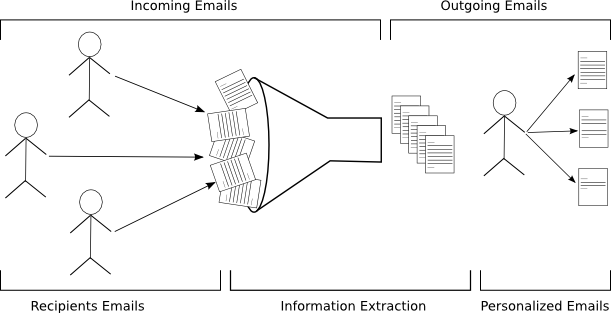
\includegraphics[width=1.00\textwidth]{imgs/drawingStatesOfEmailCommunication.png}
	\caption[Illustration of a Personalized Mass Email Communication]{Illustration of a Personalized Mass Email Communication}
	\label{fig:drawingStatesOfEmailCommunication}
\end{figure}

The information will be extracted from the recipients' emails and then a researcher will compose personalized emails for each recipient, according to the extracted information. Therefore, the discussed features of Myriad and their benefits can be grouped under the handling of the incoming emails and the outgoing email as follows:
\vspace{1cm}

\paragraph{Handling The Incoming Emails} \mbox{}\\

Myriad has a campaign inbox view to avoid cluttering of unrelated messages in the inbox, fetching only the campaign related emails from the user's email account by ignoring private emails, and grouping each email according to the campaign it belongs to.
\vspace{1cm}

As a researcher reads the incoming emails, he or she can also record the extracted information from those emails into \ac{KVP}s at the same time. This avoids the need on using a third-party application like a spreadsheet. However, if a researcher prefers a traditional way in recording information like a spreadsheet, Myriad still offers an option in synchronizing those \ac{KVP}s with a Google Spreadsheet.
\vspace{1cm}

Assistants can help a researcher with appropriate given permission on extraction of information from incoming emails.

\paragraph{Handling The Outgoing Emails} \mbox{}\\

Myriad provides a threaded view of all the email conversations of a recipient in a campaign letting researchers consider the earlier conversations with a recipient, without having the need to browse through other views. This saves time and helps on getting a quick overview of the conversation history to get a better context on personalizing the succeeding new messages.
\vspace{1cm}

The researchers can continue on using his or her own Gmail's account on answering or initiating a conversation. Myriad offers Gmail label synchronization to import those emails into a campaign, and make them more manageable along with other campaign emails.
\vspace{1cm}

The researchers can opt to reuse previously written emails as a template in composing new emails. The provided template tree also gives a direct visualization of the current campaign state and flow to let the researcher easily go through earlier given answers.
\vspace{1cm}

The researchers can use the recorded \ac{KVP}s to personalize the outgoing emails. Since personalization has been addressed as an important factor in increasing response rates, the initiated campaign will end up with better results compared to non-personalized emails.
\vspace{1cm}

Myriad records the previous actions of a user as a rule in the system to notify the automation of the email sending process with the matching conditions of a group of recipients. This helps to save time and increase awareness of the researcher to previously taken actions for repeated or similar situations.
\vspace{1cm}

Assigned assistants can also help the primary researcher in composing emails or proofreading the composed emails before they get sent out to their respective recipients.

In the next section, we will see the conclusion of this study and the possible extensions on the requirements of Myriad as a future work.

\begin{comment}

-- type of the campaigns
-- date vs number of campaign
-- date vs number of users
-- campaign Vs number of recipients
- ignore test campaigns but mention it

--> Gmail labellari ni anlatirken, diger urunlerde import nasil email forwardingle yapiliyordu onu anlat kesin.


However, we still needs to supply a system, where it offers a workflow to make it happen. satisfy these 

distribution of the work

initial idea is reducing effort as we disscussed


Requirements'dan once urunu tanit screenshot'larla cunku cok zaman kaybedecen


write first about the revised requirements,
then describe the product with pictures,
then some technical details


-------------
chapter 6 Conclusion and Future Work
-------------
Evaluation
- Experiences
- Statistics
- Conclusion

\end{comment}
